%
\section{Selection}

\subsection{Dataset}
This analysis uses all the \pp collision data in Run 1 and  Run 2 stages, corresponding to an integrated luminosity of 9\invfb. 
The simulation samples of the $\Bpdecay$ decay{\footnote{Inclusion of charge conjugation is implied throughout this note.}} are generated by \pythia
with $pp$ collisions, with \pythia8 generator.
%to produce these Monte Carlo samples. 
The Monte Carlo event type is \texttt{12145051}, in which $\Bp$ is forced to decay into the $\jpsi\phi\Kp$ final state with the PHSP(phase space) model. The statistics and simulation version is show in Table~\ref{table:MC}
 
\begin{table}[h]
\centering
\caption{The statistics and simulation version of MC. MU is magnet up, MD is magnet down.}\label{table:MC}
\begin{tabular}{ccc}
\hline
year & statistics(MU/MD) & simulation version\\
\hline \hline
2011 &      754500/766498         & Sim08c     \\
2012 &      1004812/1003052       & Sim09b     \\
2016 &      1147294/1013030       & Sim09b     \\
2017 &      1004122/1014701       & Sim09f     \\
2018 &      1008192/1000411       & Sim09f     \\
\hline
\end{tabular}
\normalsize

\end{table}   
%
\subsection{Reconstruction and pre-selection}
In this analysis the reconstruction of the \Bp candidate starts
from the stripping line \texttt{FullDSTDiMuonJpsi2MuMuDetachedLine} in the \texttt{DiMuon} stream. The stripping version of each dataset is listed in Table~\ref{stripping}. 
The selection criteria in this stripping line did not vary in different years, and are summarized in Table~\ref{tab:JpsiSelection}.
The \jpsi candidate is formed by two oppositely charged tracks consistent with muon hypotheses (IsMuon) with $\pt>500\mev$ and good track fit quality $\chisqndf<4$. 
The $\jpsi$ candidate is required to have an invariant mass within the $\pm100\mev$ window around the know \jpsi mass\supercite{PDG}, and to have a vertex fit quality $\chisqvtx<20$. 
The $\jpsi$ candidate is consistent with originating from $b$-hadron decays by requiring its decay length significance (DLS) to be greater than three. 


\begin{table}[t]
\centering
\caption{stripping version}
\begin{tabular}{cc}
\hline
year & stripping version \\
\hline \hline
2011 & Stripping21r1     \\
2012 & Stripping21       \\
2015 & Stripping24r1     \\
2016 & Stripping28r1     \\
2017 & Stripping29r2     \\
2018 & Stripping34      \\
\hline
\end{tabular}
\normalsize
\label{stripping}
\end{table}


\begin{table}[tbh]
\caption{Stripping selections of $\jpsi$ candidates in the line \texttt{FullDSTDiMuonJpsi2MuMuDetachedLine}.}
\centering
\begin{tabular}{rl}
\hline
Quantity               & Selections \\
\hline
IsMuon$(\mu)$          & $=$ TRUE \\
$\dllmupi$     & $>$ 0\\
$\pt(\mu)$             & $>500\mev$ \\
Track $\chisqndf(\mu)$ & $<3$  \\
$\Delta M(\jpsi)$      & $<100\mev$\\
Vertex $\chisq(\jpsi)$ & $<20$ \\
DLS($\jpsi$)           & $>3$  \\
\hline
\end{tabular}
\label{tab:JpsiSelection}
\end{table}

%
To select good $\jpsi$ candidates, 
vertex fit $\chi^2$ is required to be less than 9, 
and the dimuon invariant mass window is reduced to $[-57,\,43]\mev$ around the known \jpsi mass\supercite{PDG}.
The \jpsi mass resolution is around $13\mev$.  
The asymmetric window is used to take FSR of muons into account.
To reconstruction the \Bp candidate, 
the $\jpsi$ candidate is combined with two positively and one negatively charged tracks, 
all consistent with kaons.
This is achieved by PID cuts on the \ProbNN variables: $\ProbNN{\rm k}(K)>0.1$ (\texttt{MC12TuneV3} for Run 1 and \texttt{MC15TuneV1} for Run 2, respectively). 
The kaon candidate is required to have transverse  momentum, 
$\pt>250\mev$, and detached from the primary vertex (PV) with impact parameter (IP) satisfying $\chisqip>4$. 
The three kaon candidates are required to come from the same vertex with good vertex-fit quality, $\chisq<50$ for $ndf=3$.
The $\Bp$ candidate is required to have a displaced decay vertex, 
with flight distance (FD) more than 1.5\mm and  form a good vertex with fit quality, $\chisqndf<9$.
%    displaced vertex by requiring $\chisq_\tau>9$, 
It should be consistent with being produced from PV by requiring $\chisqip<20$ and cosine value of the angle with respect to PV, DIRA$>0.99$. 
The $\Bp$ candidates with mass $4.9<M(\jpsi \phi \Kp)<5.7 \gev$ are preselected.  
To reject clone tracks, 
any two tracks in $\Bp$ candidate have an opening angle smaller than 0.5\,mrad are removed. 
%The preseletion efficiency on signal MC is {\color{red} xx\%}.

The $\Bpdecay$ decay chain is refitted with two sequential constraints using the \texttt{DecayTreeFitter} to improve the mass resolution: 
A) the \jpsi candidate mass constrained to its known value\supercite{PDG} and 
the $\Bp$ candidate constrained to originating from the associated PV; 
%resulting in a better resolution of the $\Lb$ invariant mass. 
B) the invariant mass of the $\Bp$ candidate constrained to  the know $\Bp$ mass value\supercite{PDG}, 
with the momenta of the $\jpsi$ and kaon daughters re-calculated according to this constraint. 
For amplitude fits discussed later, 
the updated daughter four-momenta are used to calculate invariant masses and angles.  

Then, 
at least one of the two $K^+K^-$ combined mass to be within $\pm15$\mev of the known $\phi$ mass is required\supercite{PDG}.
and only one $\phi$ candidate is accepted for further analysis. 
To be more specific, 
candidates that have two $K^+K^-$ combinations with mass falling into the $\pm15$\mev window are abandoned. 
This reduces the sample by about 3\%. 
To be consistent with quantities used in amplitude analysis, 
the $\phi$ candidate mass is recalculated with kaon four-momenta after all kinematic constraints. 
All the selection criteria are summarized in Table~\ref{tab:PreSelection}. 

%
It should be noted that the PID requirements on the hadron tracks are not applied when reconstructing the $\Bp$ candidates in the simulation sample.
The effect, instead, is reconsidered after correcting the PID distributions in simulation using the PID calibration (\texttt{PIDCorr}). 

Events with $\Bp$ candidates in both the simulation and the data samples are required to fire any level-zero trigger line and to be of TOS type with respect to at least one high level trigger lines listed in Table \ref{trigger}.

\begin{table}[h]
\centering
\caption{Tigger requirements on $\Bp$ candidates.}
\begin{tabular}{c|c|c}
\hline
     & Run 1 & Run 2 \\
\hline
L0 &  \multicolumn{2}{c}{Global\_DecDecision}  \\
\hline
\multirow{4}{*}{Hlt1 TOS} & \multicolumn{2}{c}{TrackMuon} \\
& \multicolumn{2}{c}{DiMuonHighMass }                            \\
& TrackAllL0 & TrackMVA \\
& &  TwoTrackMVA \\
                       \hline
\multirow{3}{*}{Hlt2 TOS} &\multicolumn{2}{c}{TopoMu2,3,4Body}\\
&\multicolumn{2}{c}{DiMuonDetachedJPsi}\\
&\multicolumn{2}{c}{DiMuonDetachedHeavy}\\
\hline
\end{tabular}
\normalsize
\label{trigger}
\end{table}

%%%%%%%%%%%%%%%%%%%%%%%%%%%%%%%%%%%%%%%%%%%%%%%%%%%%%%%%%%%%%%%%%%%%%%%%%%%%%%%%%%%%%%%%%%%%%%%%%%%%%%%%%%%%%%%%%%%%%%%

%%%%%%%%%%%%%%%%%%%%%%%%%%%%%%%%%%%%%%%%%%%%%%%%%%%%%%%%%%%%%%%%%%%%%%%%%%%%%%%%%%%%%%%%%%%%%%%%%%%%%%%%%%%%%%%%%%%%%%%

%%%%%%%%%%%%%%%%%%%%%%%%%%%%%%%%%%%%%%%%%%%%%%%%%%%%%%%%%%%%%%%%%%%%%%%%%%%%%%%%%%%%%%%%%%%%%%%%%%%%%%%%%%%%%%%%%%%%%%%
\begin{table}[tbh]
\caption{All pre-selections of $\Bpdecay$ candidates including stripping and offline levels.}
\centering
\begin{tabular}{lll}
\hline
Candidate & Quantity                & Selections  \\
\hline
All tracks & Track fit $\chisqndf$ & $<3$\\
All tracks & Ghost prob & $<0.47$\\

\hline
$\mu$ & IsMuon          & $=$ TRUE \\
$\mu$ & $\dllmupi$     & $>$ 0\\
$\mu$ & $\pt$             & $>500\mev$ \\\hline

$\jpsi$  & mass window& $\in(-57,43)$\mev\\
$\jpsi$ & Vertex $\chisq$ & $<9$ \\
$\jpsi$ & DLS           & $>3$  \\\hline

$K$& $\ProbNN{\rm k}$        & $>0.1$ \\
$K$ & $\pt$            & $>250\mev$ \\
$K$& $\chisqip$       & $>4$ \\
$3K$ & Vertex $\chisqndf$ & $<50/3$\\\hline
$\phi$ & mass window & $\pm15$\mev\\
\hline
$\Bp$ & Vertex $\chisq$ & $<9$ \\
$\Bp$ & FD    & $>1.5$\mm   \\
$\Bp$ & $\chisqip$         & $<20$   \\
$\Bp$ & $DIRA$             & $>0.99$   \\
$\Bp$ & $M$   & $\in(4.9,5.7)\gev$   \\
$\Bp$ & Opening angle of two tracks &$>0.5$\,mard\\
$\Bp$ & \# of $\phi$ candidate & $=1$\\
\hline
\end{tabular}
\label{tab:PreSelection}
\end{table}
%%%%%%%%%%%%%%%%%%%%%%%%%%%%%%%%%%%%%%%%%%%%%%%%%%%%%%%%%%%%%%%%%%%%%%%%%%%%%%%%%%%%%%%%%%%%%%%%%%%%%%%%%%%%%%%%%%%%%%%

%
\subsection{Multivariate analysis}
The multivariate analysis (MVA) is used to further suppress the backgrounds. 
The signal training sample is from the 
${B}^{+} \rightarrow {J} / {\psi} {\phi} {K}^{+}$ simulation using the PHSP model, 
while the background sample is from the invariant-mass sidebands of ${B}^{+} \rightarrow {J} / {\psi} {\phi} {K}^{+}$ data sample, 
with $M(\jpsi \phi K^+)\in[5.229,5.254] \cup [5.304,5.329]\gevcc$.
These samples are randomly split into two halves, 
one for the training and the other one for the test.

The following variables are used in the MVA: the log of $\chi^2_{IP}$ of B;
the log of minimum of ProbNNk among the three kaons;
the DIRA of B;
the $\chi^2_{vertex}/\mathrm{dof}$ of B;
the $\pt$ of B;
the $\pt$ sum of three kaons;
the $\chi^2_{FD}$ of B;
the log minimum $\chi^2_{IP}$ of kaons.
The distributions of these variables for the signal in the simulation sample and for the background in the data $\Bp$ sidebands are shown in Figure.~\ref{fig:MVAvairables_run1} (Run 1) and Figure. ~\ref{fig:MVAvairables_run2} (Run 2). 


\begin{figure}[!tbp]
\centering
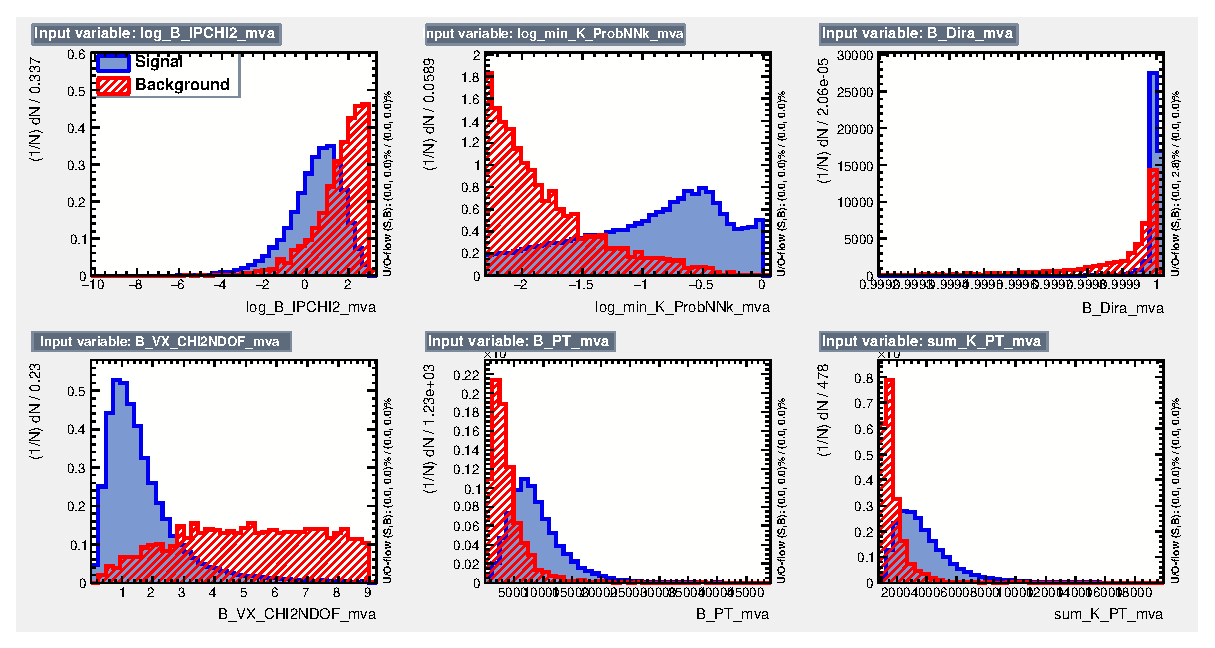
\includegraphics[width=0.8\textwidth]{Figures/03_Zcs/04_Selection/variables_id_c1_run1}
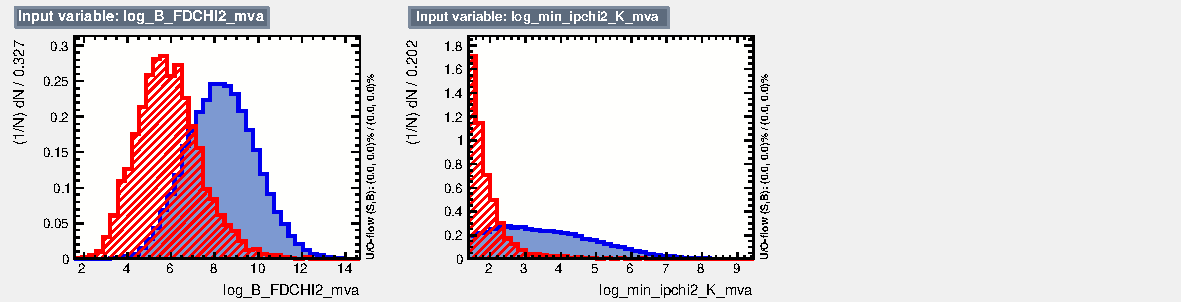
\includegraphics[width=0.8\textwidth]{Figures/03_Zcs/04_Selection/variables_id_c2_run1-1}
\caption{Discriminating variables used in the MVA training for Run 1} 
\label{fig:MVAvairables_run1}
\end{figure}

\begin{figure}[!tbp]
\centering
%\begin{minipage}[t]{0.8\textwidth}
%\centering
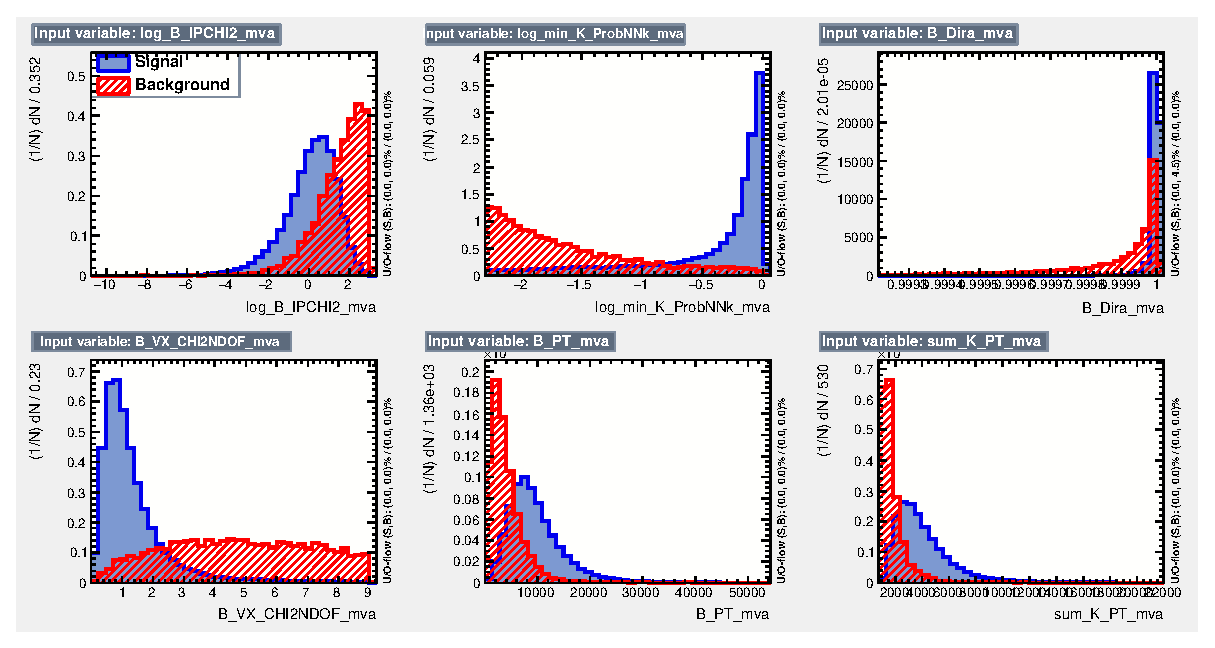
\includegraphics[width=0.8\textwidth]{Figures/03_Zcs/04_Selection/variables_id_c1_run2}\\
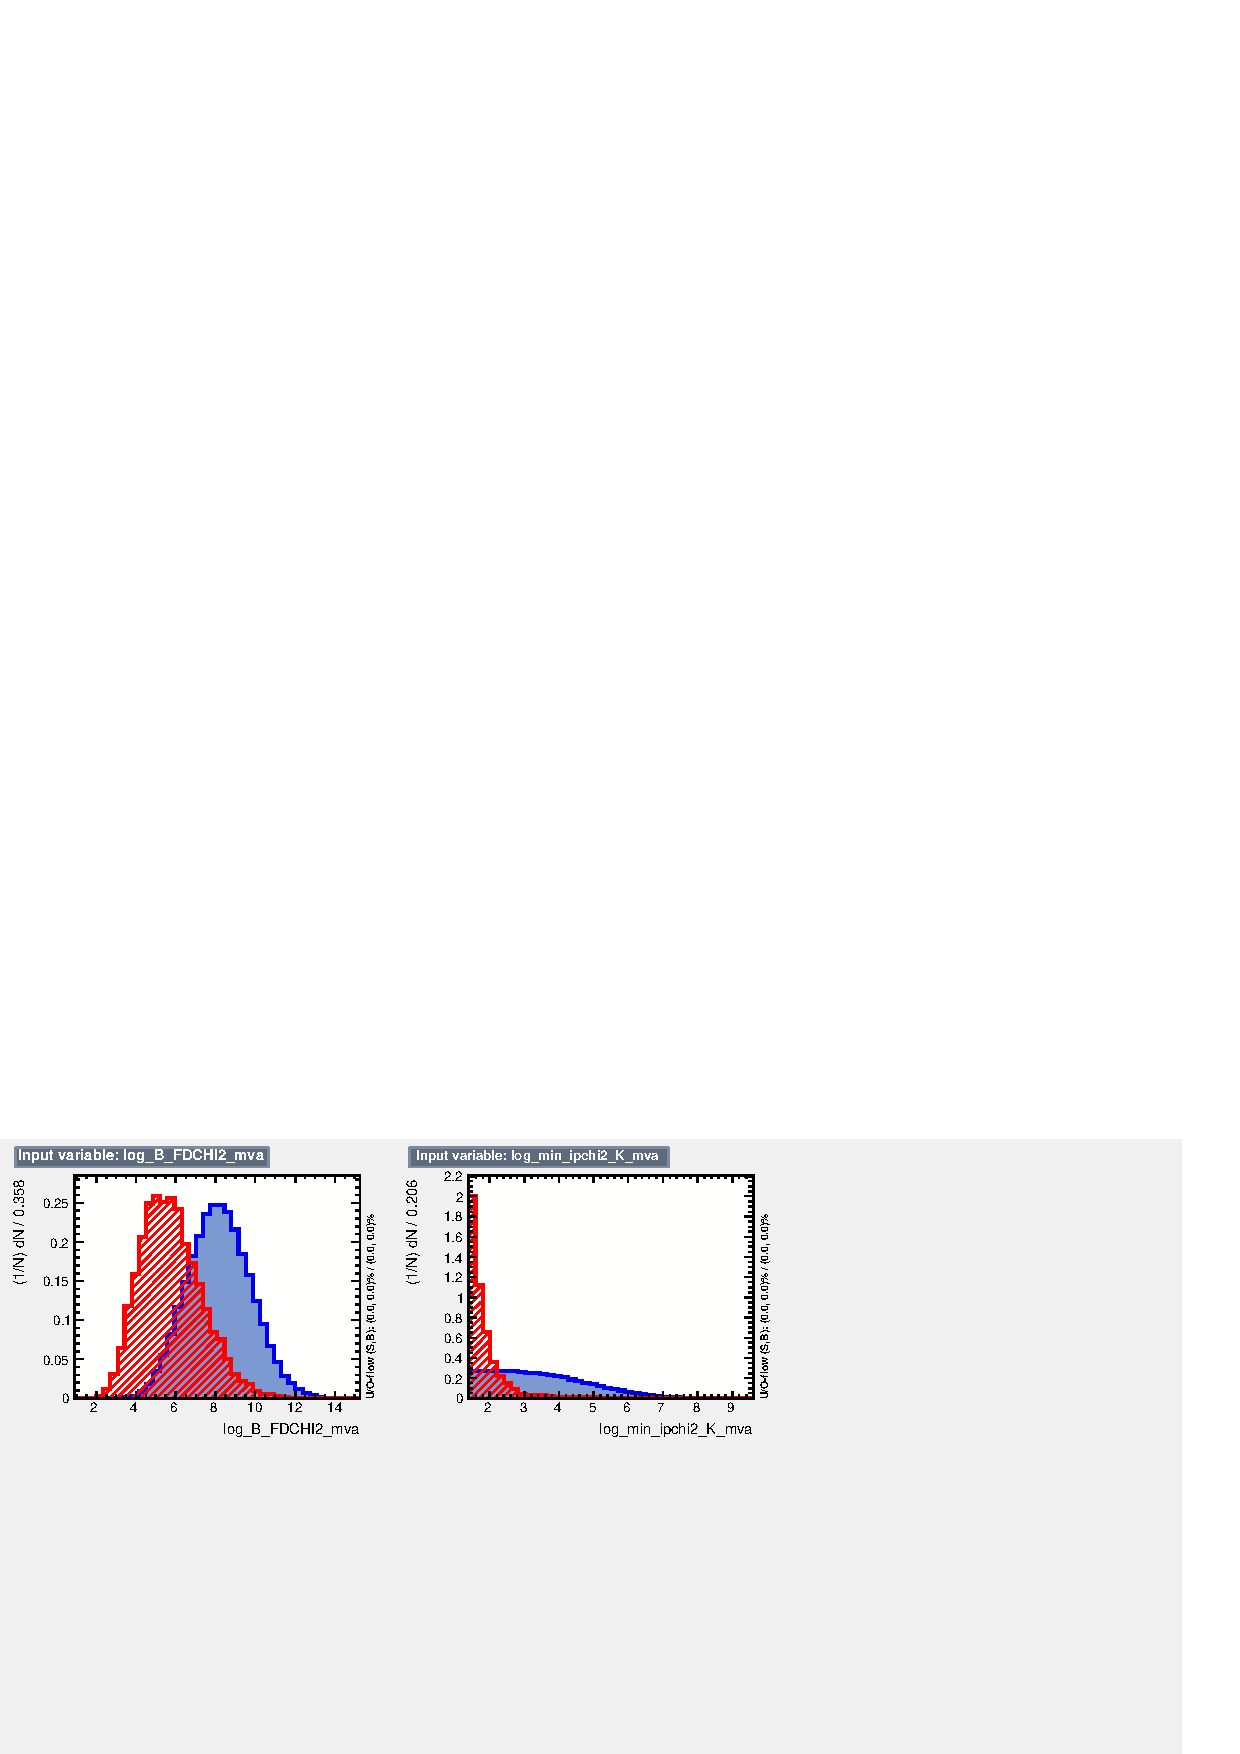
\includegraphics[width=0.8\textwidth]{Figures/03_Zcs/04_Selection/variables_id_c2_run2-1}
%\end{minipage}
\caption{Discriminating variables used in the MVA training for Run 2} 
\label{fig:MVAvairables_run2}
\end{figure}

For Run 1, The ROC curves of the results of different training methods are given in the left plot of Figure.~\ref{fig:MVAMonitor_run1}.  
The BDTG method is used as the default method, 
and the overtraining test for the BDTG method is given for Run 1 in the right plot of Figure.~\ref{fig:MVAMonitor_run1}. 
The BDTG discriminant distributions for the training samples are consistent with those in the test samples. 
No effect of overtraining is observed.
Similar results for Run 2 are given in Figure.~\ref{fig:MVAMonitor_run2}. 

%The working point of the BDTG value is optimized by maximizing the figure of merit (FoM) of the signal significance, defined as 
%$\frac{S}{\,sqrt{S+B}} \times \frac{S}{S+B}$. 
A 2D scan of BDTG value and cut on track-ghost probability for the kaons is done to maximize the figure of merit (FoM) of the signal significance, 
defined as $\frac{S}{\sqrt{S+B}} \times \frac{S}{S+B}$.  
%The $\epsilon_S$ is the signal efficiency for a specified BDTG cut and is determined from the simulation sample, while 
$S$ ($B$) is the number of the signal (background) events in the $\pm2.5\sigma$ region around the known $B$ mass in the
 $\jpsi\phi K^+$ invariant mass distribution of the data. 
%It should be noted that the PID requirements on the $p$ and $\pi$ need also to be tightened on top of the pre-selection. 
%However, it is found that the BDTG cut value that maximizes the FoM doesn't depends strongly on the PID cuts of the two hadron tracks. 
In Figure.~\ref{fig:BDTGCut_run1} (Figure.~\ref{fig:BDTGCut_run2}), 
the distribution of the FoM as a function of the BDTG cut value and 
the track-ghost probability for kaons are given for Run 1 (Run 2). A BDTG cut value of $>0.15$ ($>-0.14$) and 
the track-ghost probablity for kaons of $<0.47$ ($<0.40$) are determined as the default working point for Run 1 (Run 2).

%The PID requirement on the proton is tightened slightly to $\ProbNN_p>0.2$ to further suppress the background and retain a high efficiency of the signal selection. 
%Because it is found that tighter requirement will reduce significant amount of signals,
%so no tighter requirement is applied on the proton PID. The PID requirement on the $\pi$ track is efficient to suppress the CKM favoured decay \LbJpsipK, which is an avoidable background component. 
%A cut on the combined PID variable, $\ProbNN_{\pi}\times(1-\ProbNN_{K})>0.5$ is applied to the $\pi$ track, which suppresses the background to a reasonable level, and leaves about $90\%$ of the signals on top of the pre-selection. The efficiency of the additional
%PID requirements is about $81\%$ for signals.

%%%%%%%%%%%%%%%%%%%%%%%%%%%%%%%%%%%%%%%%%%%%%%%%%%%%%%%%%%%%%%%%%%%%%%%%%%%%%%%%%%%%%%%%%%%%%%%%%%%%%%%%%%%%%%%%%%%%%%%
%%%%%%%%%%%%%%%%%%%%%%%%%%%%%%%%%%%%%%%%%%%%%%%%%%%%%%%%%%%%%%%%%%%%%%%%%%%%%%%%%%%%%%%%%%%%%%%%%%%%%%%%%%%%%%%%%%%%%%%

%%%%%%%%%%%%%%%%%%%%%%%%%%%%%%%%%%%%%%%%%%%%%%%%%%%%%%%%%%%%%%%%%%%%%%%%%%%%%%%%%%%%%%%%%%%%%%%%%%%%%%%%%%%%%%%%%%%%%%%
\begin{figure}[!tbp]
\begin{minipage}[t]{0.48\textwidth}
\centering
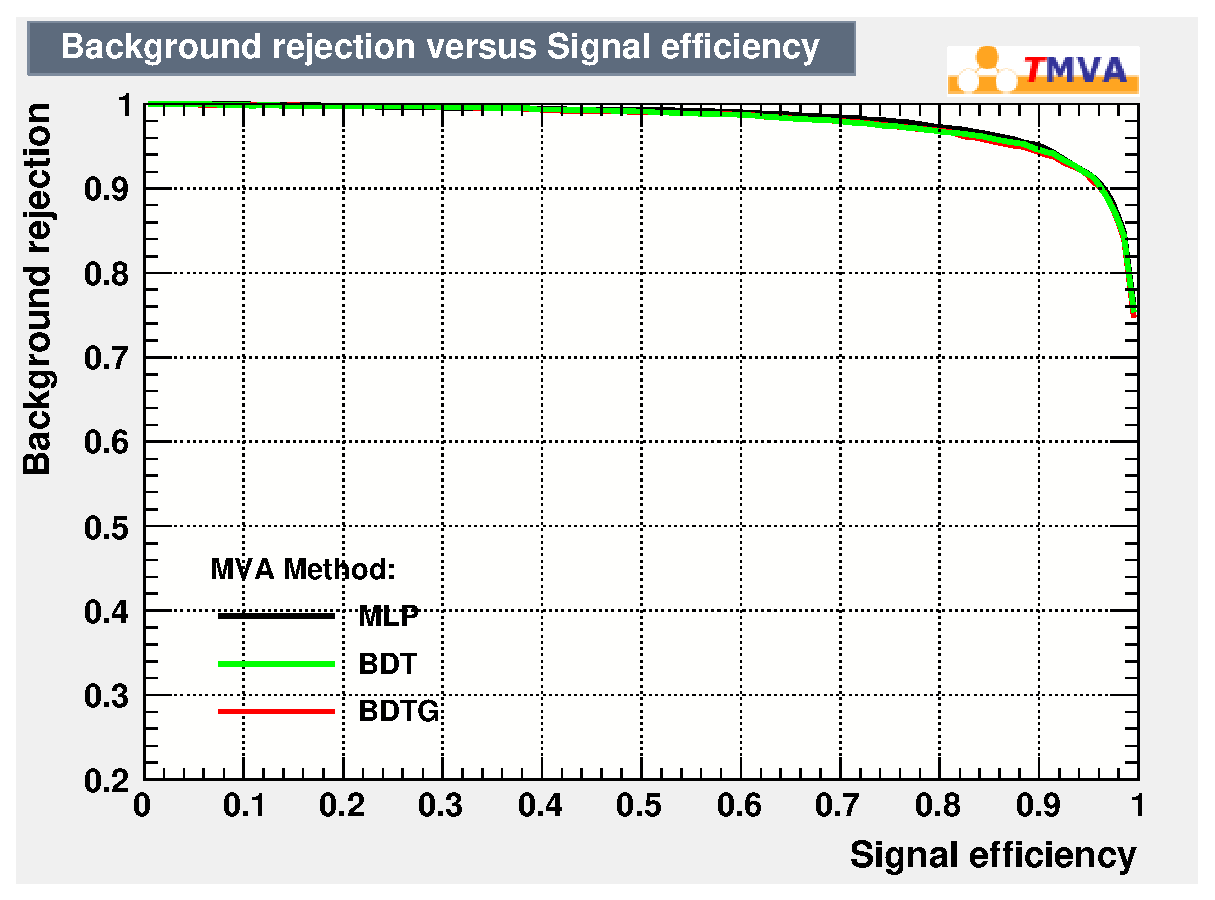
\includegraphics[width=1.0\textwidth]{Figures/03_Zcs/04_Selection/rejBvsS_run1}
\end{minipage}
\begin{minipage}[t]{0.48\textwidth}
\centering
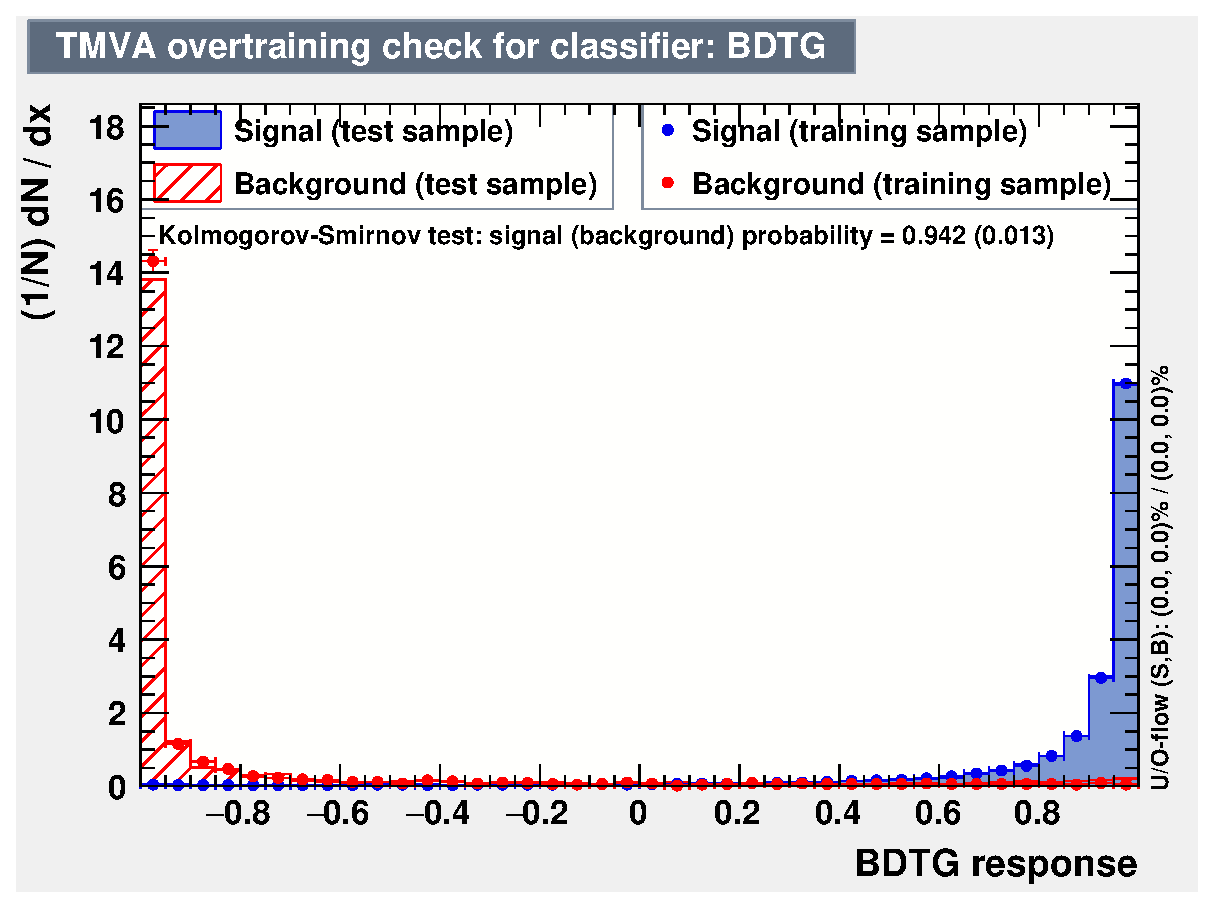
\includegraphics[width=1.0\textwidth]{Figures/03_Zcs/04_Selection/overtrain_BDTG_run1}
\end{minipage}
\caption{ 
 (left) ROC curves for different MVA methods and (right) the BDTG output distribution for signals and the background in the training sample and the test sample for Run 1.} 
\label{fig:MVAMonitor_run1}
\end{figure}

\begin{figure}[!tbp]
\begin{minipage}[t]{0.48\textwidth}
\centering
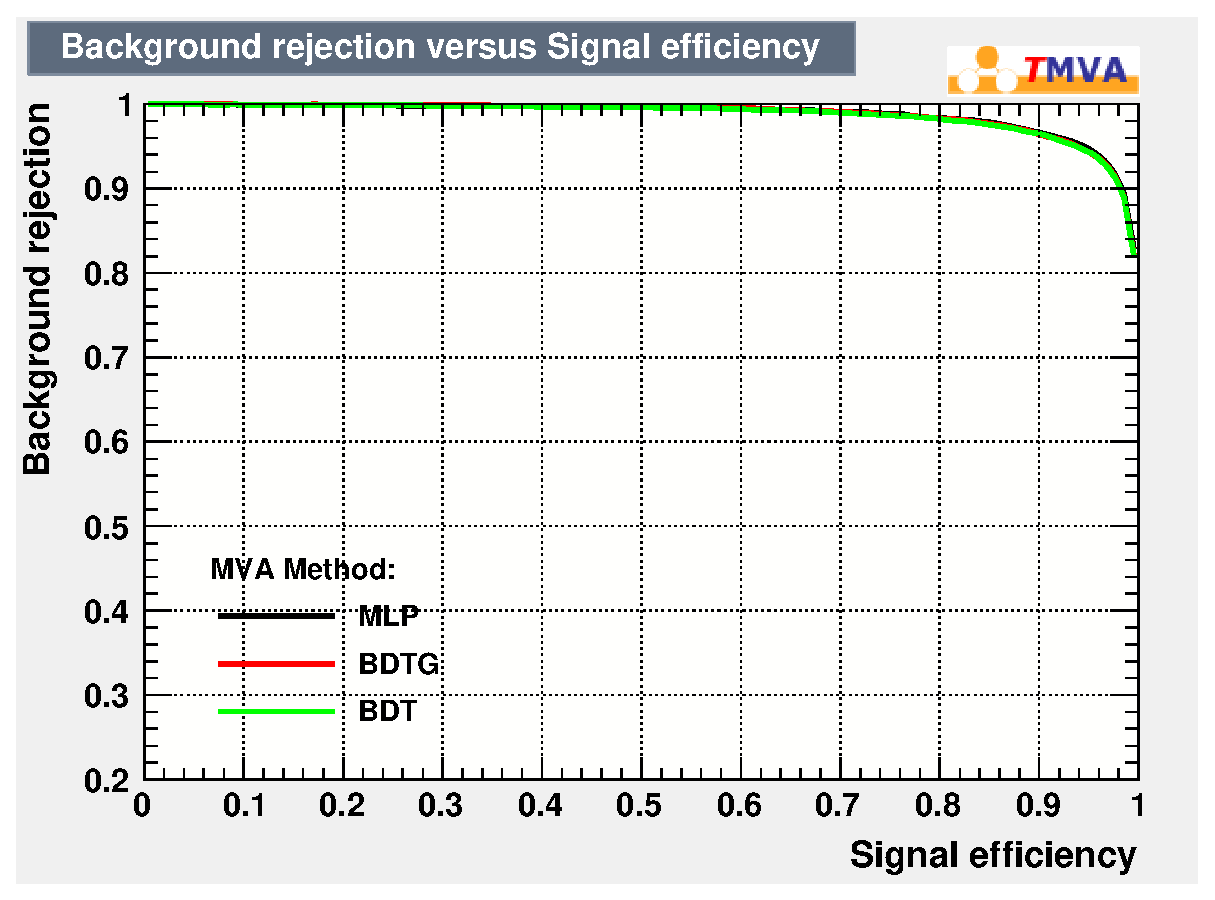
\includegraphics[width=1.0\textwidth]{Figures/03_Zcs/04_Selection/rejBvsS_run2}
\end{minipage}
\begin{minipage}[t]{0.48\textwidth}
\centering
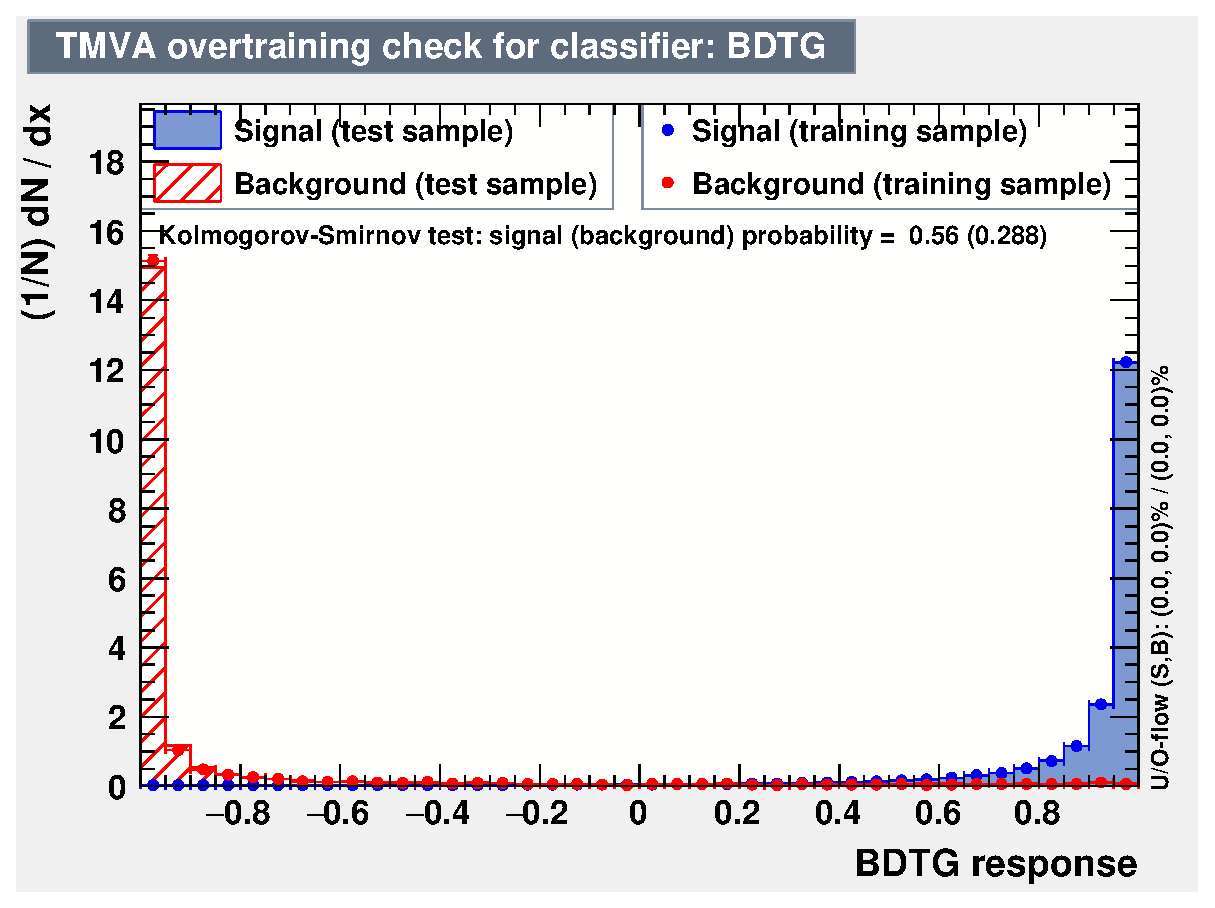
\includegraphics[width=1.0\textwidth]{Figures/03_Zcs/04_Selection/overtrain_BDTG_run2}
\end{minipage}
\caption{ 
 (left) ROC curves for different MVA methods and (right) the BDTG output distribution for signals and the background in the training sample and the test sample for Run 2.} 
\label{fig:MVAMonitor_run2}
\end{figure}

\begin{figure}[!tbp]
\centering
\begin{minipage}[t]{0.6\textwidth}
\centering
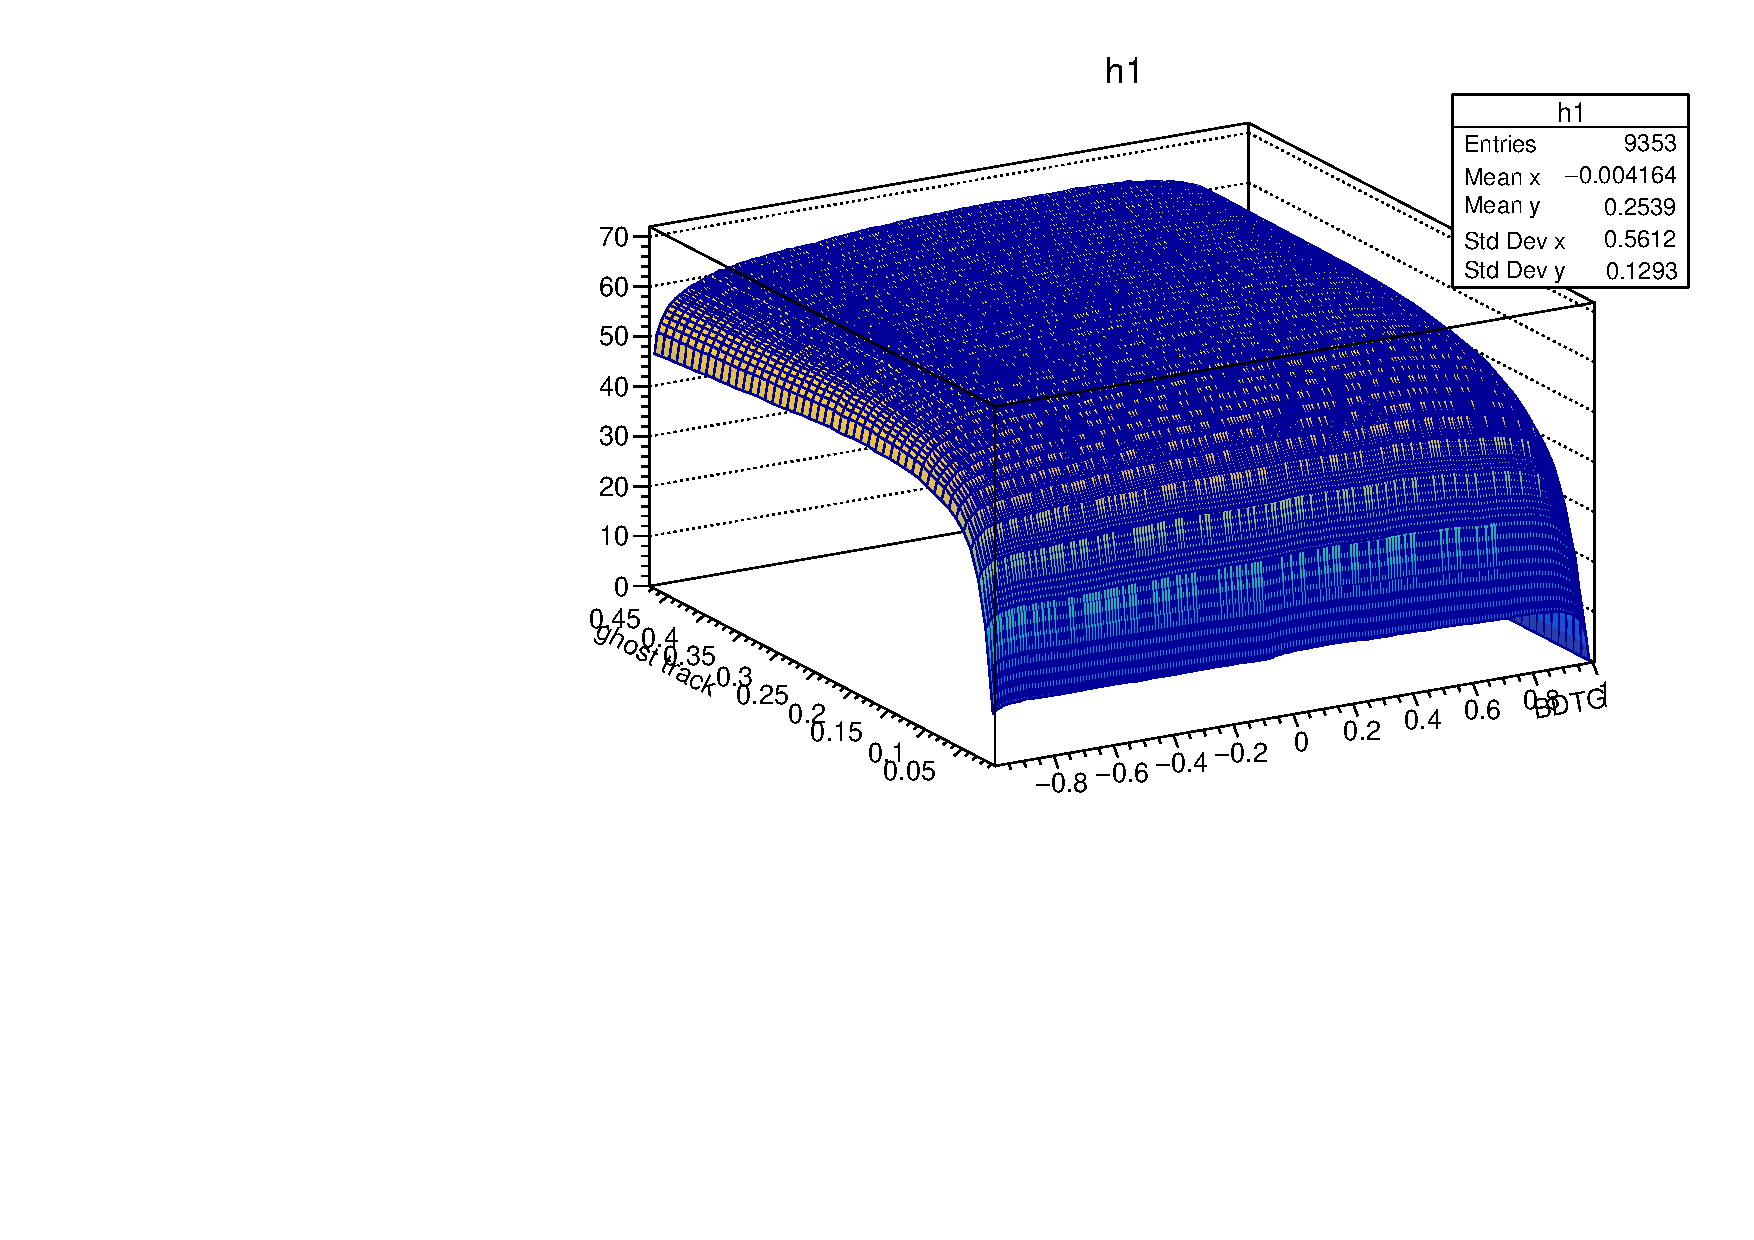
\includegraphics[width=1.0\textwidth]{Figures/03_Zcs/04_Selection/significance_run1}
\end{minipage}
\caption{Signal significance (arbitrary units) for different cuts on BDTG and track-ghost probablity for kaons for Run 1.} 
\label{fig:BDTGCut_run1}
\end{figure}

\begin{figure}[!tbp]
\centering
\begin{minipage}[t]{0.6\textwidth}
\centering
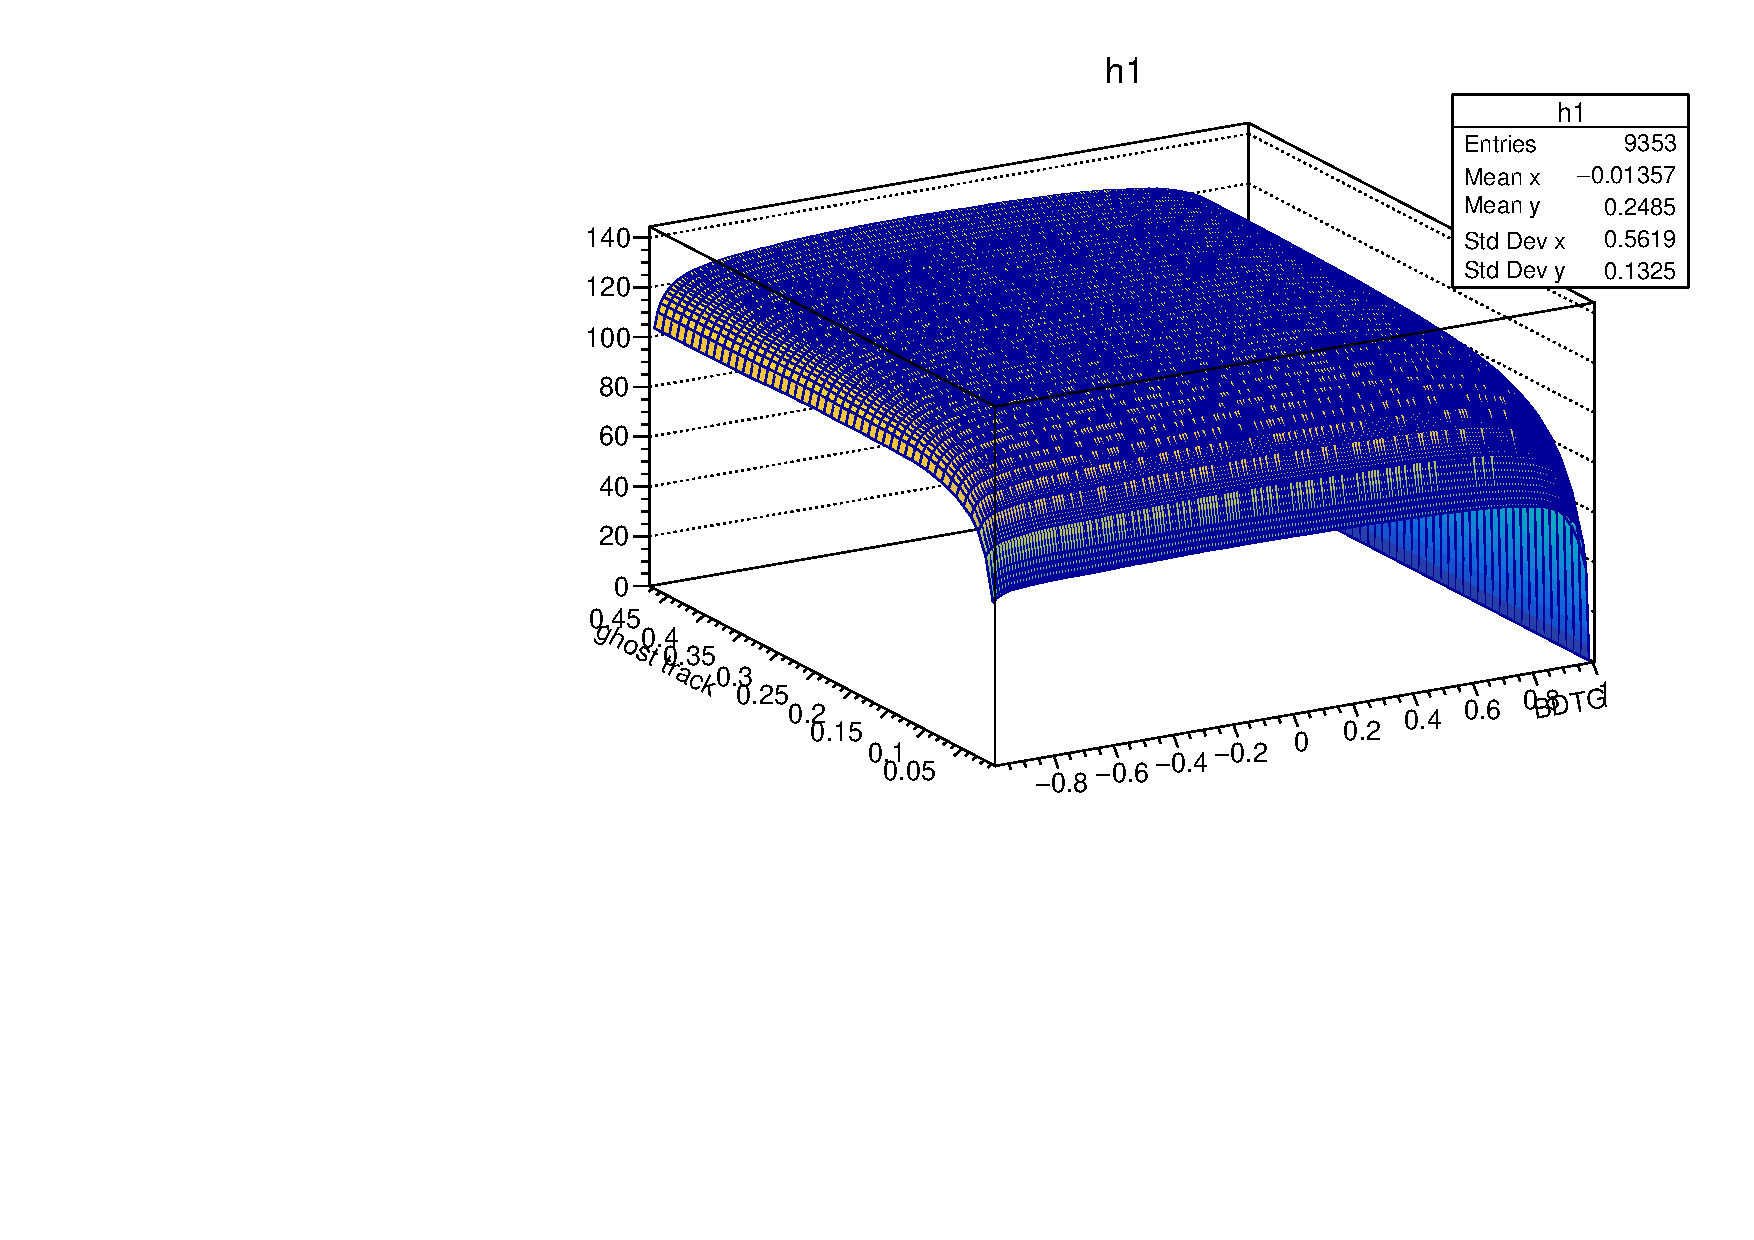
\includegraphics[width=1.0\textwidth]{Figures/03_Zcs/04_Selection/significance_run2}
\end{minipage}
\caption{Signal significance (arbitrary units) for different cuts on BDTG and track-ghost probablity for kaons for Run 2.} 
\label{fig:BDTGCut_run2}
\end{figure}
%%%%%%%%%%%%%%%%%%%%%%%%%%%%%%%%%%%%%%%%%%%%%%%%%%%%%%%%%%%%%%%%%%%%%%%%%%%%%%%%%%%%%%%%%%%%%%%%%%%%%%%%%%%%%%%%%%%%%%%

\begin{figure}[!tbp]
\centering
   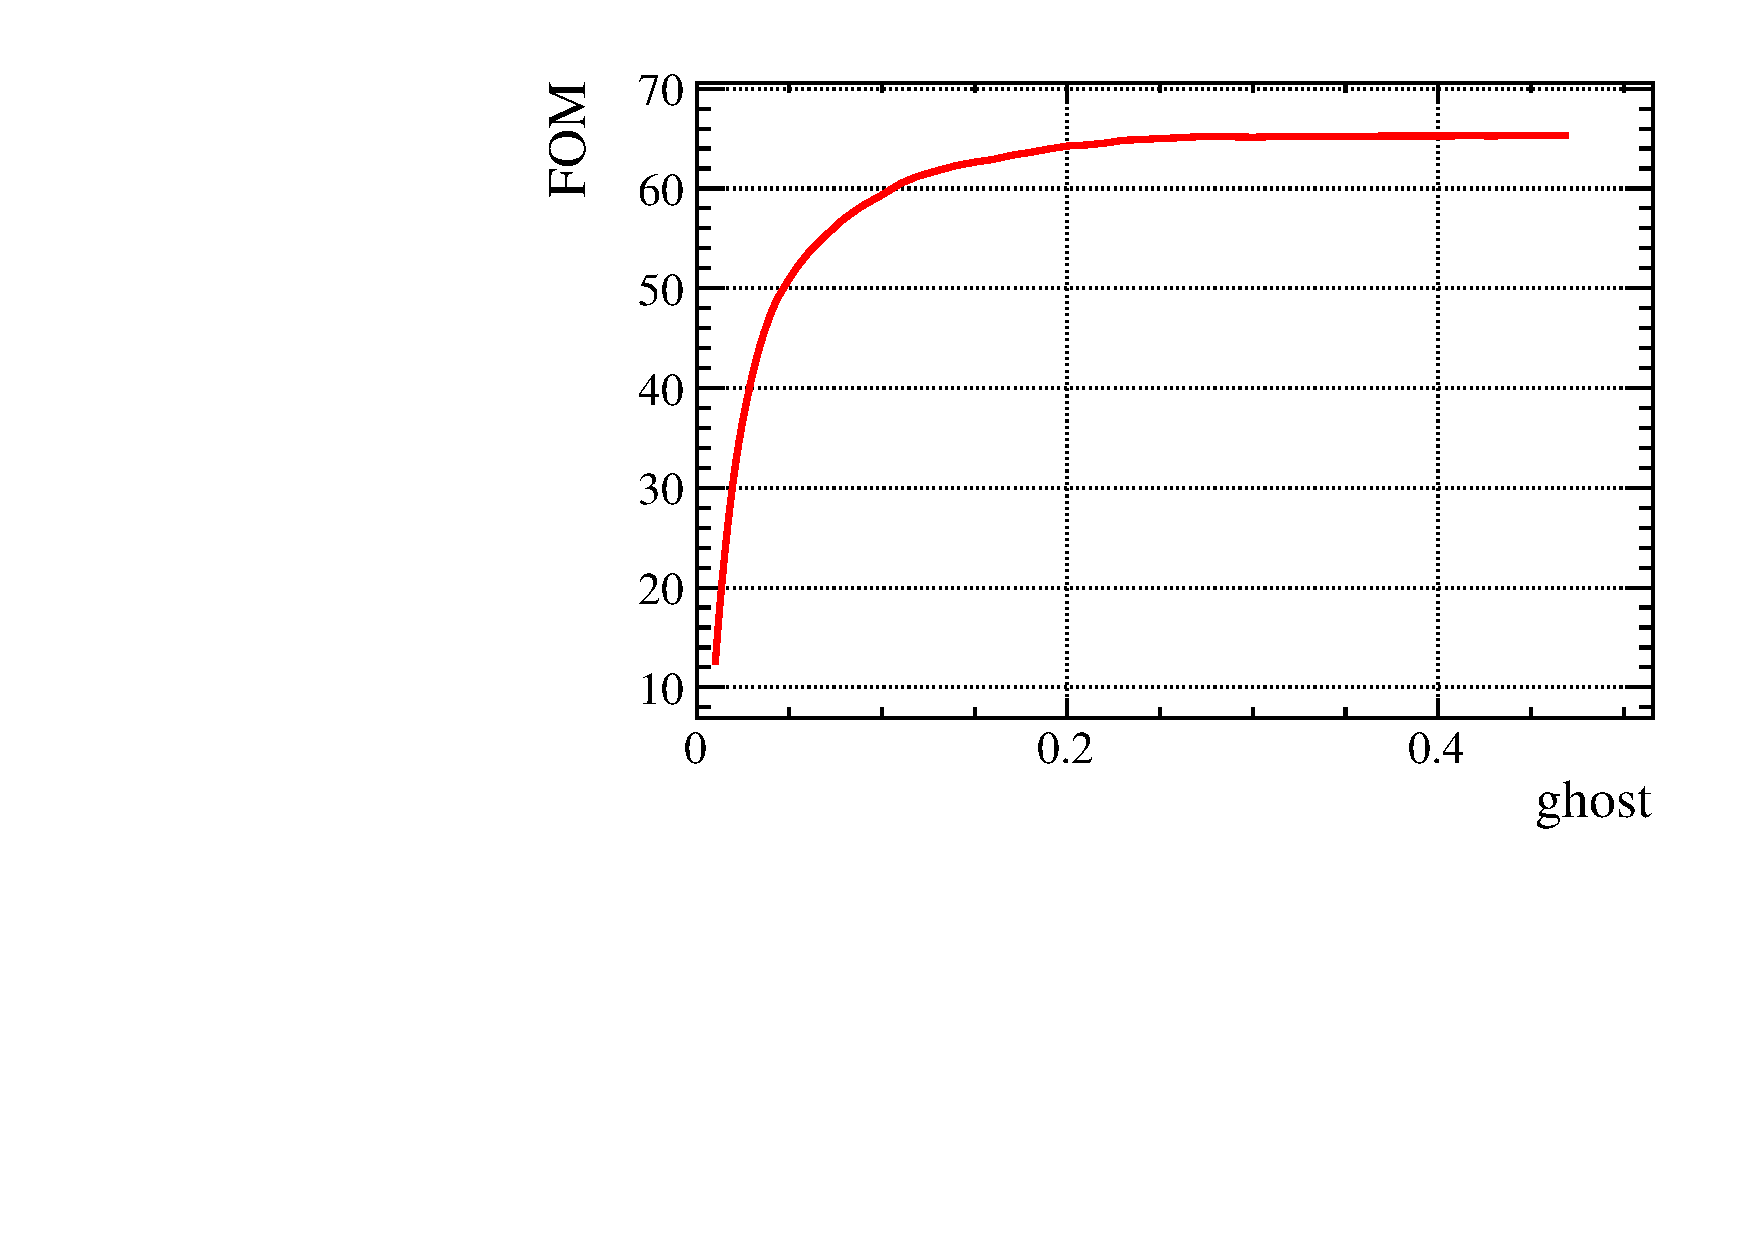
\includegraphics[width=0.5\textwidth]{Figures/03_Zcs/04_Selection/FOM/BDTG_FOM_BDTGfixed0.15_run1.pdf}
\put(-120,100) {run1 BDTG$>0.15$}
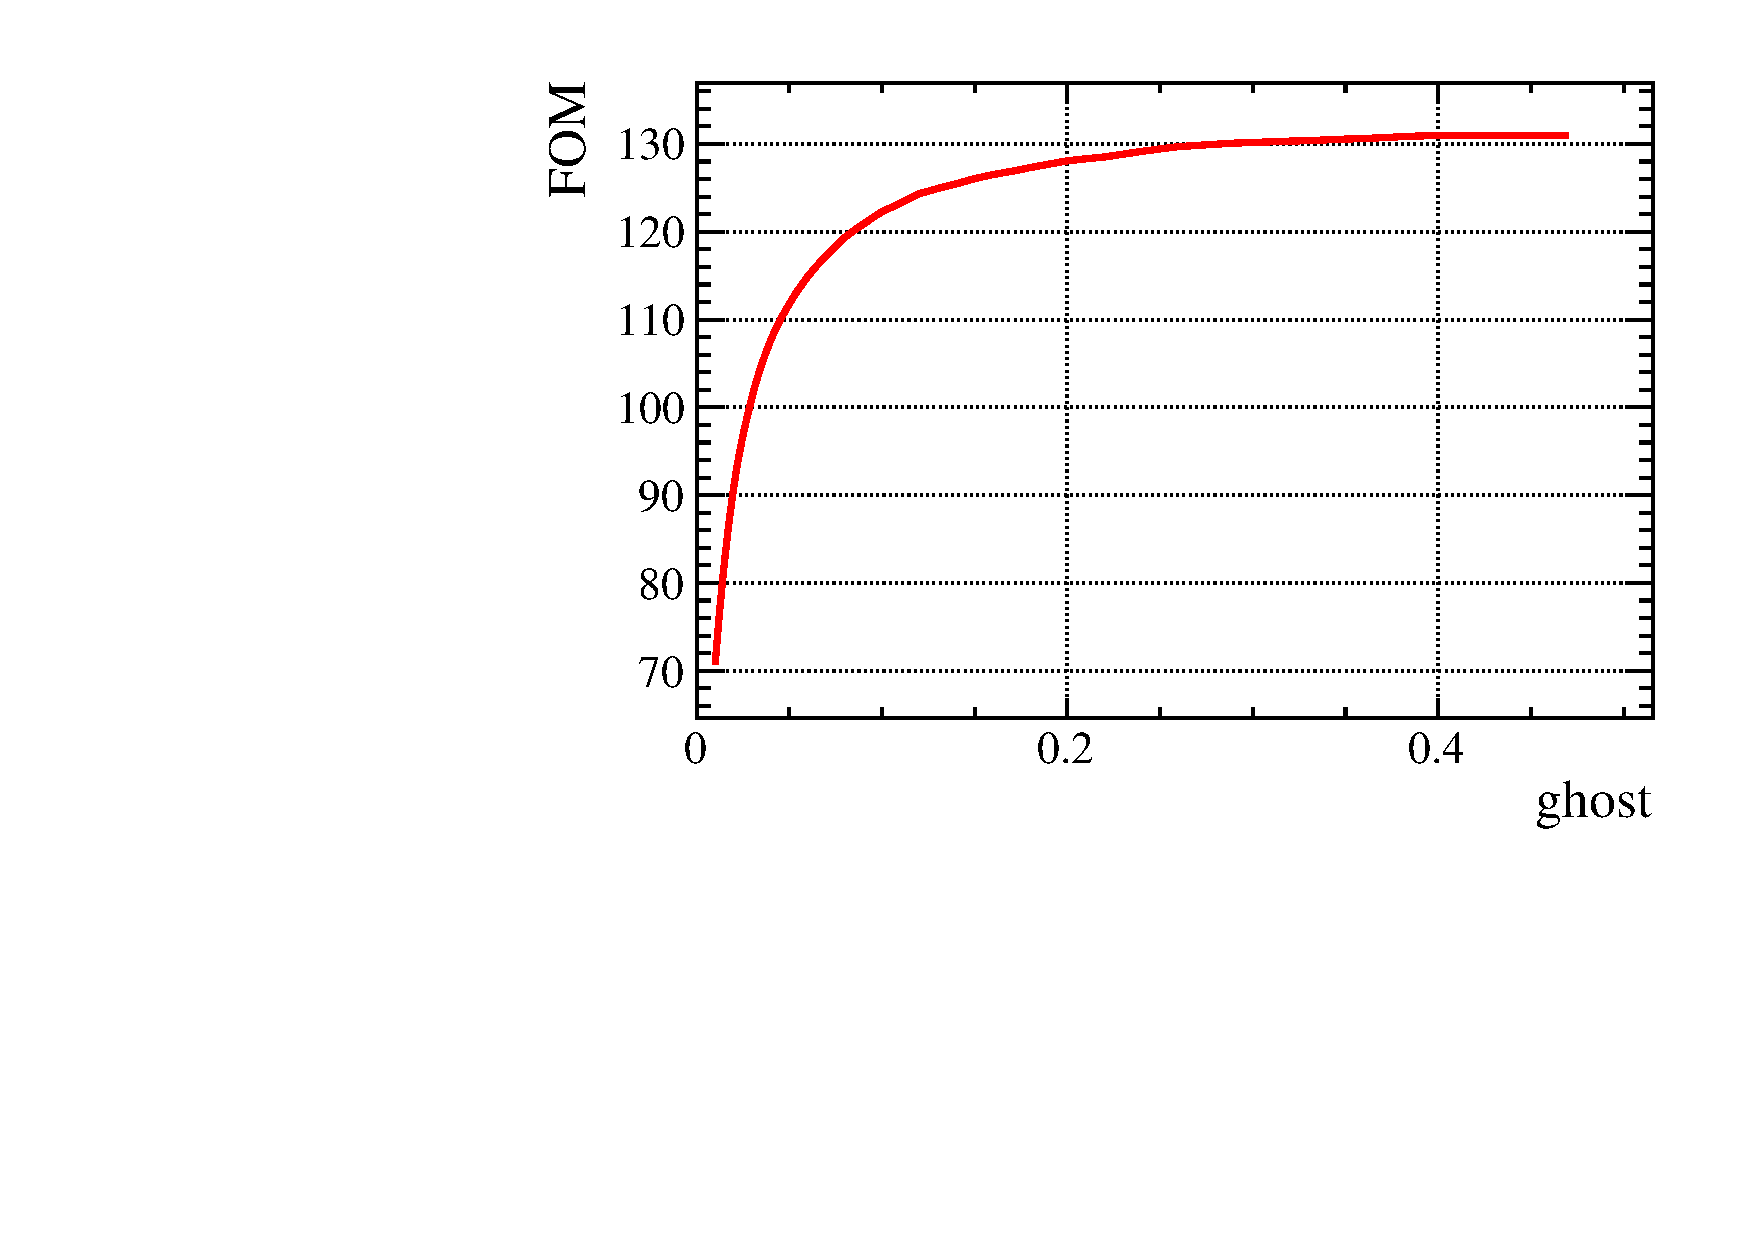
\includegraphics[width=0.5\textwidth]{Figures/03_Zcs/04_Selection/FOM/BDTG_FOM_BDTGfixed-0.14_run2.pdf}
\put(-120,100) {run2 BDTG$>-0.14$}\\
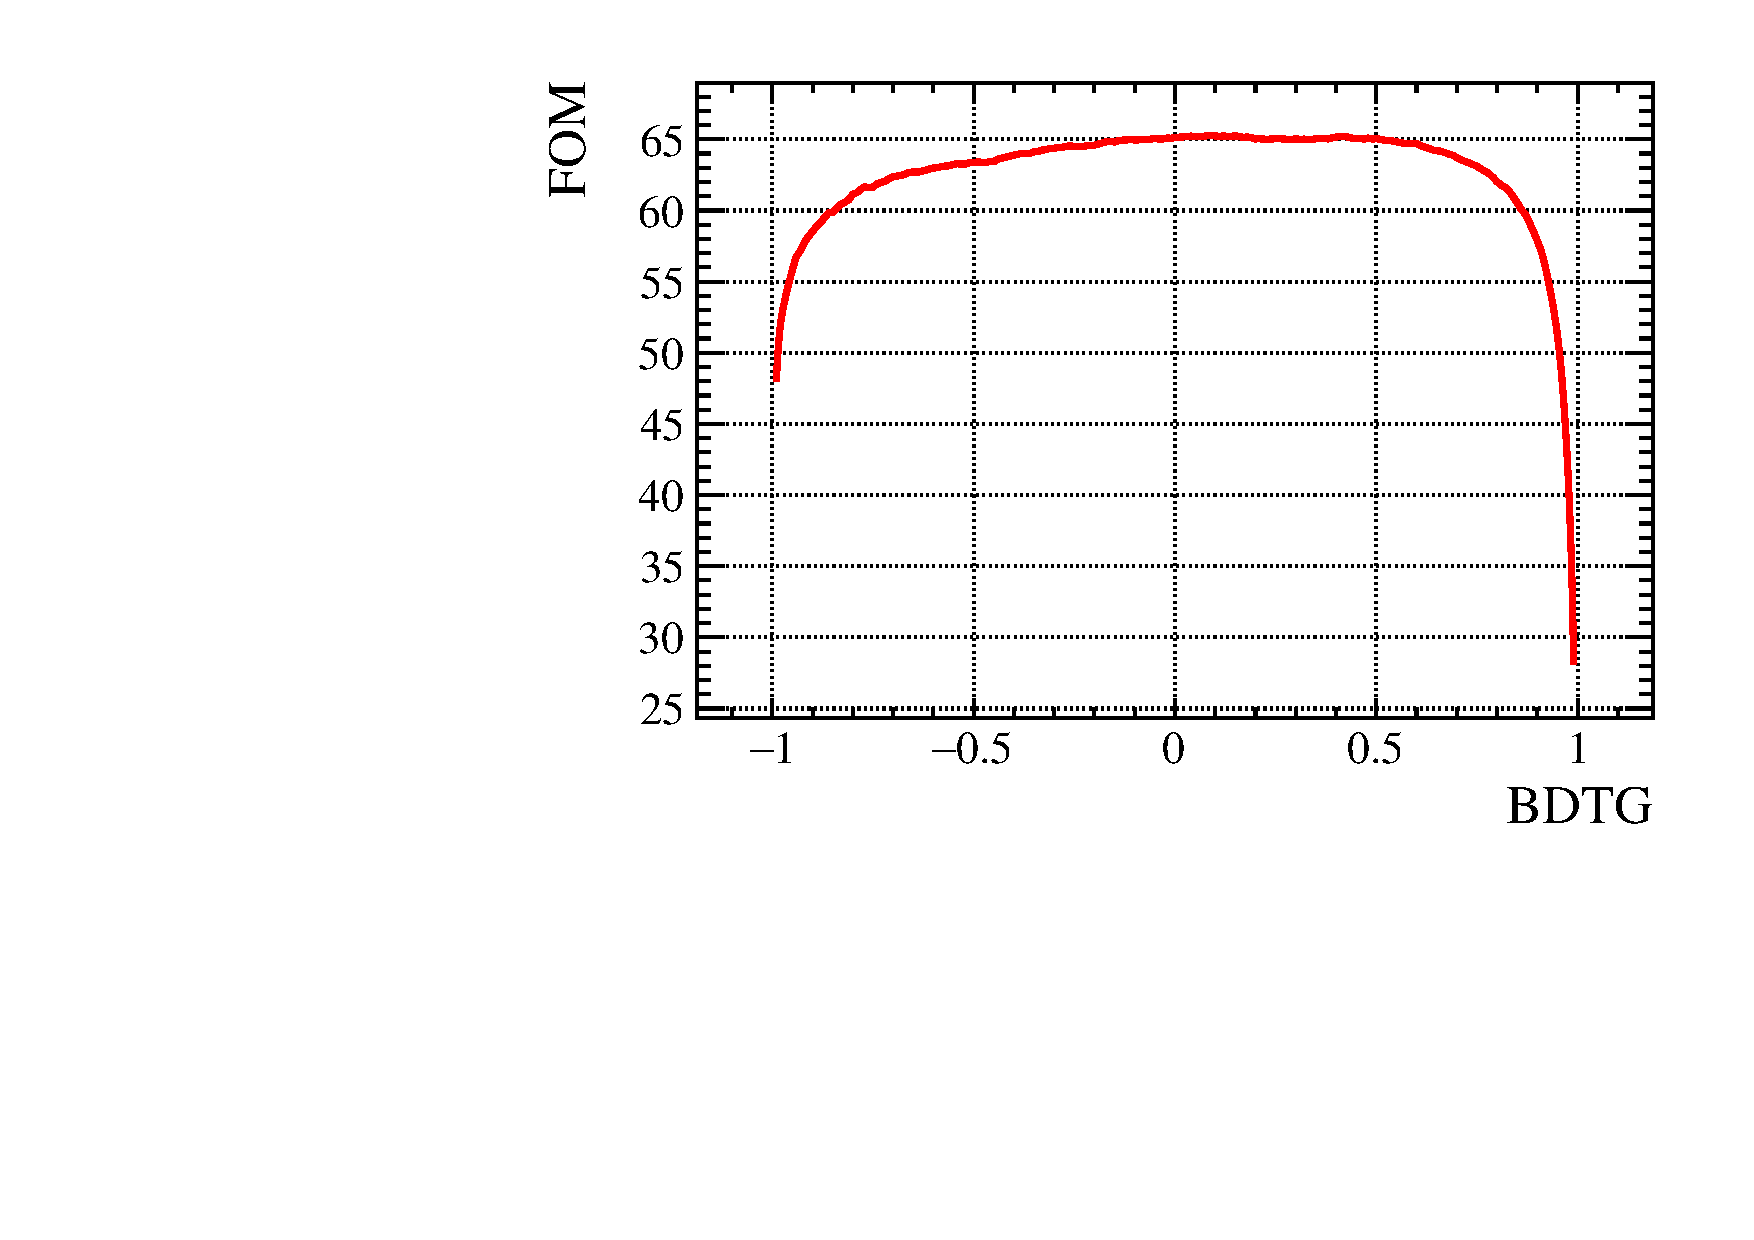
\includegraphics[width=0.5\textwidth]{Figures/03_Zcs/04_Selection/FOM/BDTG_FOM_ghostfixed0.4_run1.pdf}
\put(-120,100) {run1 ghost$<0.4$}
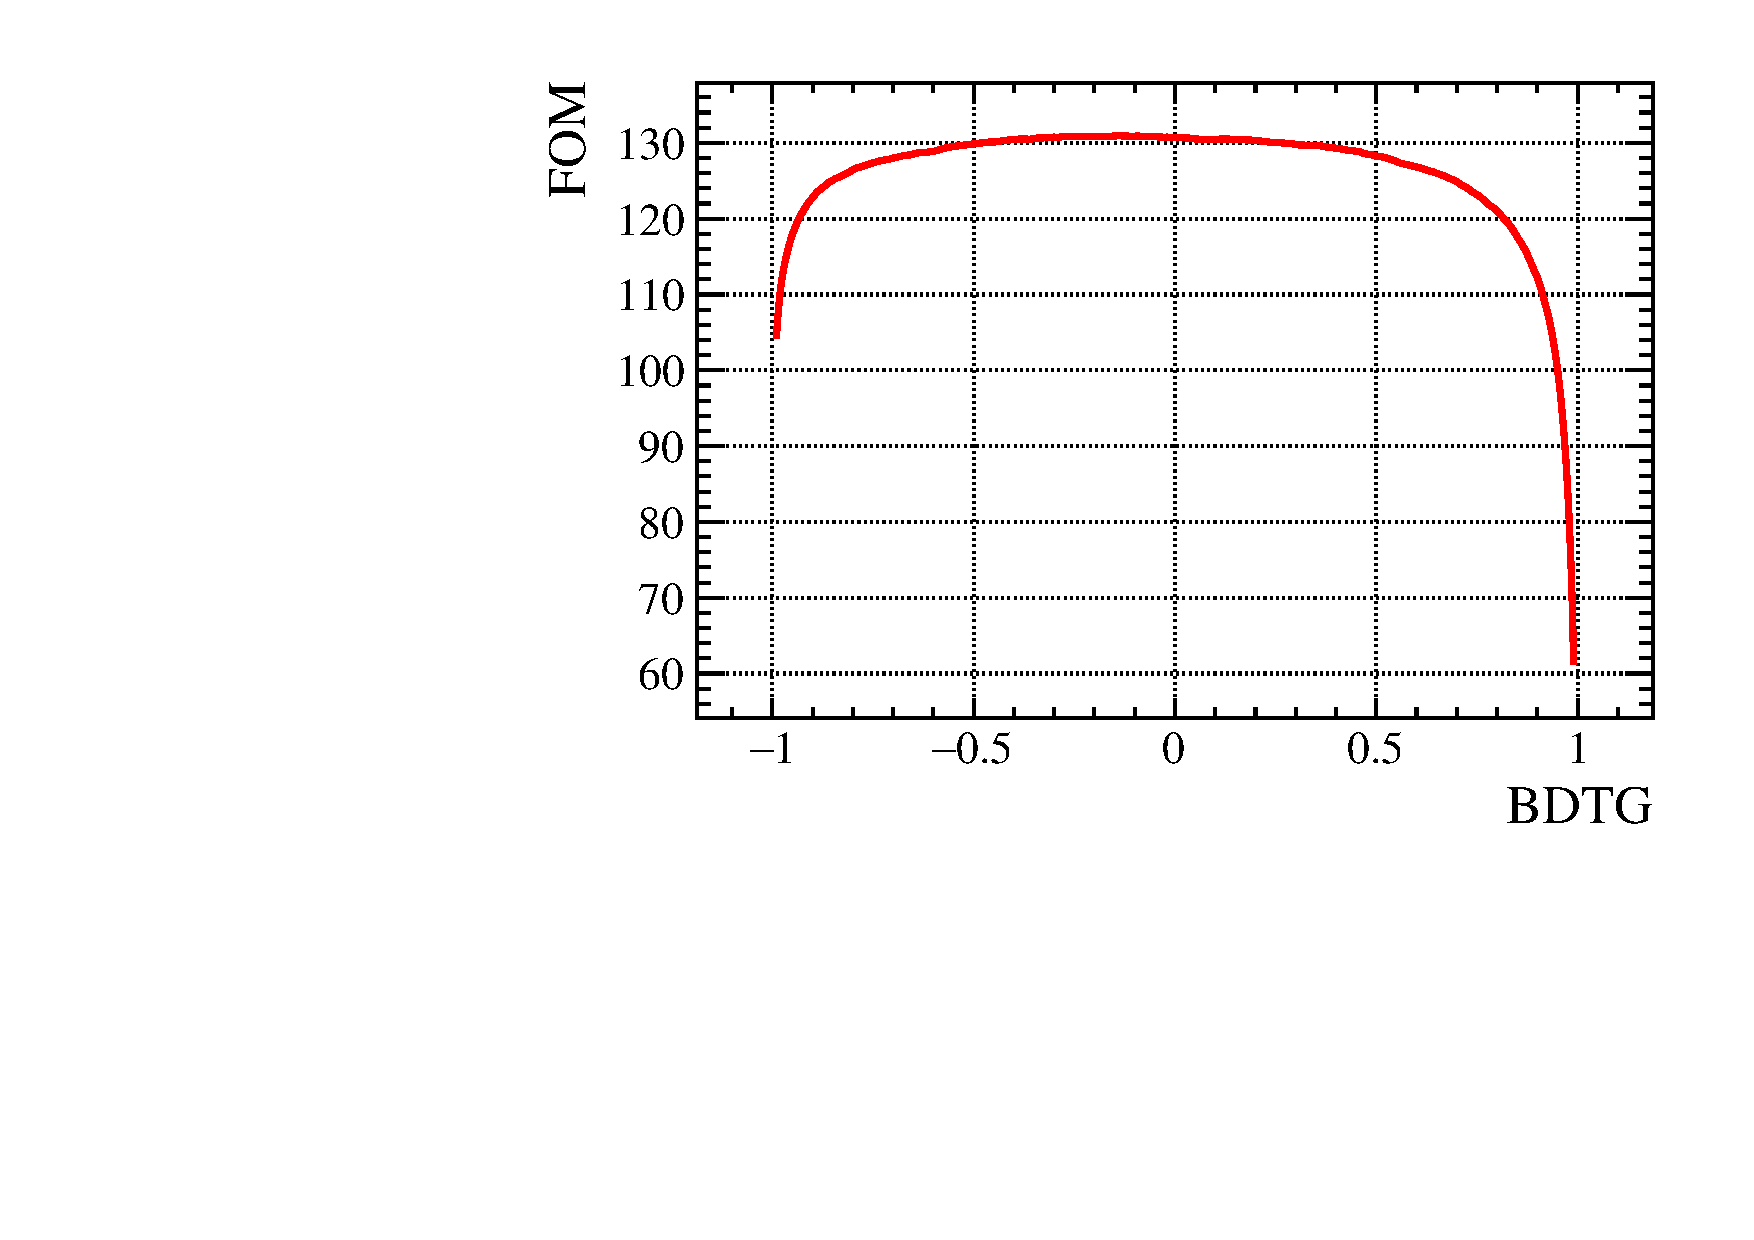
\includegraphics[width=0.5\textwidth]{Figures/03_Zcs/04_Selection/FOM/BDTG_FOM_ghostfixed0.47_run2.pdf}
\put(-120,100) {run2 ghost$<0.47$}
\caption{FOM versus BDTG, FOM versus ghost probability of kaons for run1 and run2} 
\label{fig:BDTGCut_ghost_fixed}
\end{figure}

